\chapter{Hướng tiếp cận}

% \cite{laina2016deeper}
% abcde \cite{Ma2017SparseToDense} abcd \cite{ICF}


Ở chương này, nhóm sẽ trình bày chi tiết về mô hình ước lượng độ sâu được nhóm sử dụng cũng như các kĩ thuật liên quan.
% giới thiệu lại dùng mask-rcnn với cách tính khoảng cách gọn thôi
Ở giai đoạn ước lượng khoảng cách vật thể , nhóm sẽ sử dụng ảnh độ sâu có được ở mô hình trên và Mask RCNN\cite{He2017MaskR} thông qua các phương pháp mà nhóm đề xuất để mỗi vật thể được nhận diện trong ảnh RGB sẽ có khoảng cách tương ứng.

% Trong quá trình luận văn, nhóm sẽ tiếp cận vấn đề với 2 hướng
% \begin{itemize}
% \item Thực hiện bao đóng 3D vật thể dựa vào 2D proposals
% \item Từ bao đóng 2D, thực hiện matching model để phát hiện hình dáng của vật thể.
% \end{itemize}
\begin{comment} 
\section{Mô hình cơ bản}


Mô hình để dự đoán khoảng cách của vật thể sẽ dựa theo cấu trúc trên hình 5.1, được chia làm 3 nhiệm vụ: đầu tiên, ta sẽ dự đoán depth map của ảnh RGB dựa trên Fully Convolutional Residual Networks (FCRN), tiếp theo áp dụng Mask RCNN để tiến hình phát hiện, bao đóng, phân mảnh vật thể dựa trên ảnh RGB. Dựa vào kết quả của 2 mô hình trên, áp dụng các phương pháp khác nhau để có thể ước lượng được khoảng cách vật thể. 
\end{comment}

\section{Ước lượng ảnh độ sâu từ ảnh RGB}
Để dự đoán độ sâu từ một ảnh RGB, Laina et al. \cite{laina2016deeper} đã đề xuất fully convolutional residual network (FCRN), nó chỉ gồm một kiến trúc đơn nhất và được huấn luyện từ đầu đến cuối (end-to-end) mà không đòi hỏi các kĩ thuật hậu xử lí như các bước tinh chỉnh kết quả (refinement step). Sau đó, nhằm cải thiện độ tin cậy và chính xác của kết quả dự đoán độ sâu chỉ sử dụng một ảnh đơn. Ma et al. \cite{Ma2017SparseToDense} đã xây dựng mạng CNN có cấu trúc dựa trên FCRN, nhưng sử dụng một ảnh độ sâu thưa cùng với ảnh RGB để tái tạo lại một ảnh độ sâu có độ phân giải cao. Ảnh độ sâu thưa có thể được sinh ra từ các depth sensor có chi phí thấp, hoặc được tính toán bằng giải thuật Simultaneous Localization and Mapping (SLAM) như \cite{SLAM}. Đây chính là hướng tiếp cận của nhóm.\\

Ở mục 4.1 này, phần đầu nhóm sẽ trình bày kiến trúc mạng FCRN (fully covolutional neural network) của \cite{laina2016deeper}, nhằm ánh xạ một ảnh RGB sang ảnh độ sâu tương ứng. Ở phần sau nhóm sẽ nói về deep regression network của Ma et al.\cite{Ma2017SparseToDense} có đầu vào là ảnh RGB kết hợp với ảnh độ sâu thưa để hướng dẫn mạng dự đoán độ sâu tại mỗi điểm ảnh.  Ma et al.\cite{Ma2017SparseToDense} đã dùng kĩ thuật lấy mẫu độ sâu (depth sampling) từ ảnh độ sâu thực để tạo ra ảnh độ sâu thưa phục vụ cho quá trình huấn luyện mạng, kĩ thuật đó sẽ được nhóm làm rõ ở đây cũng như các kĩ thuật khác như data augmentation, hàm đo độ lỗi (loss function) được sử dụng trong quá trình tối ưu. 

%\subsection{Kiến trúc của mạng CNN}
%\subsection{Fully convolutional residual network}
\subsection{Dự đoán độ sâu từ một ảnh đơn với fully convolutional residual network}
Mạng fully convolutional residual network được đề xuất bởi Laina et al. \cite{laina2016deeper} lấy ý tưởng từ residual learning để dự đoán độ sâu. Như chúng ta đã biết ở chương trước, hầu hết các mạng CNN hiện nay gồm nhiều lớp mà mỗi lớp là một phép tính convolution hoặc pooling và khi một bức ảnh RGB được đưa vào mạng thì chuỗi phép tính này sẽ liên tục làm giảm độ phân giải của nó, điều này giúp cho các nơron càng thuộc về các lớp sau sẽ có vùng thụ cảm (receptive field) tương ứng càng lớn, dẫn đến lượng thông tin toàn cục mà nó nhận được sẽ lớn hơn các lớp trước. Ước lượng độ sâu là một bài toán hồi quy (regression) nhưng đầu ra mong muốn có độ phân giải cao, nên chúng ta sẽ cần các phép up-sampling để có được đầu ra lớn hơn. Eigen\cite{Eigen2014,Eigen2015} đã dùng lớp kết nối đầy đủ (fully-connected layers) để các nơron lớp này có vùng thụ cảm chứa toàn bộ bức ảnh làm cho nó có thể hiểu toàn cục khung cảnh, điều này là cần thiết vì nó có thể sử dụng hiệu quả hơn các đặc điểm như vị trí của đối tượng, hướng của căn phòng... so với việc chỉ hiểu được những phần cục bộ của bức ảnh để đưa ra những dự đoán khoảng cách tốt hơn. Nhưng việc dùng lớp kết nối đầy đủ để dự đoán độ sâu sẽ khiến mô hình tăng số lượng tham số , do đó độ phân giải của đầu ra sẽ không lớn như mong muốn.\\

Kiến trúc của Laina et al.\cite{laina2016deeper} đã tiến hành loại bỏ lớp kết nối đầy đủ, mỗi đầu vào được tùy chỉnh về size 304$\times$228, và đầu ra mong muốn là một nửa độ lớn của đầu vào, Laina et al.\cite{laina2016deeper} đã tiến hành khảo sát một số kiến trúc nổi tiếng như AlexNet\cite{Krizhevsky2012} và VGG-16\cite{Simonyan2014} bởi vì trọng số đã huấn luyện sẵn của các mô hình này giúp cho việc hội tụ tốt hơn và thấy rằng nếu bỏ đi lớp kết nối đầy đủ thì vùng thụ cảm của lớp convolutional cuối cùng của AlexNet là 151$\times$151, của VGG-16 là 276$\times$276 nó vẫn nhỏ hơn 304$\times$228, đây là độ lớn đầu vào của chúng ta. Do đó nó chưa đủ để hiểu thông tin toàn cục của bức ảnh, nhưng với sự ra đời của ResNet\cite{KHe2015} và ý tưởng residual learning, nó giúp tạo các mạng CNN cực sâu mà vẫn cho kết quả tốt hơn các mạng thông thường, đồng thời các mạng này có vùng thụ cảm lớn hơn. Với ResNet-50 nó có vùng thụ cảm là 483$\times$483 đủ lớn để tiếp nhận toàn bộ thông tin của đầu vào. Vậy với một bức ảnh 304$\times$228 thì lớp convolutional cuối cùng của  ResNet-50 sẽ cho ra 2048 feature map có độ phân giải 10$\times$8.  Nếu chúng ta dùng lớp kết nối đầy đủ để sinh ra đầu ra có độ phân giải là 160$\times$128 thì sẽ tốn mất 3.3 tỷ tham số và nó sẽ cần đến 12.6GB trong bộ nhớ, do đó sử dụng phương pháp này là không thể so  với phần cứng hiện tại. Do đó Laina et al.\cite{laina2016deeper} đã dùng một vài phép residual up-covolution thay cho lớp kết nối đầy đủ để đạt được đầu ra có độ lớn 160$\times$128, điều này đã giúp cho mạng fully convolutional chứa ít tham số hơn cũng như cải thiện được độ chính xác của việc dự đoán độ sâu.\\

Tóm lại kiến trúc đề xuất của Laina et al.\cite{laina2016deeper} gồm 2 phần. Phần đầu của mạng là dựa trên ResNet-50 \cite{KHe2015}, nó đã bị bỏ lớp average pooling và lớp kết nối đầy đủ cuối cùng. Phần sau của kiến trúc sẽ hướng dẫn mạng học cách tăng độ phân giải của feature map bằng bốn lớp upsampling và cuối cùng là dùng phép bilinear interpolation để có độ phân giải bằng với đầu ra ban đầu.
 \begin{center}
         \begin{figure}[H]
         \begin{center}
           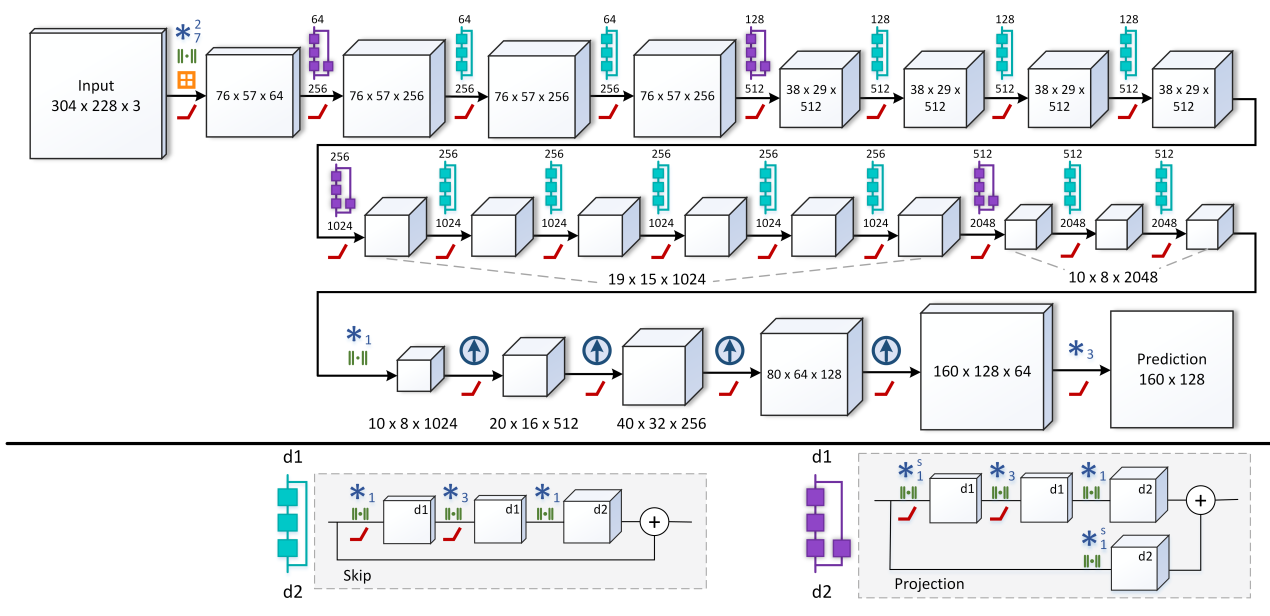
\includegraphics[scale=0.35]{image/LainaNet}
          \end{center}
          \caption{Kiến trúc của FCRN. Mỗi khối là một feature map với số chiều là $\#height\times width\times channel$, phần đầu là ResNet-50\cite{KHe2015}, output của nó là khối 10$\times$8$\times$2048 cuối cùng, sau đó là 1 lớp 1$\times$1 convolution và 4 phép upsampling, cuối cùng là 1 phép 3$\times$3 convolution để sinh ra output với độ phân giải một nửa so với input }
          \label{ref_sigmoid}
          \end{figure}
 \end{center}
% Chúng ta sẽ thiết lập để input có size là 304 x 228 và một khía cạnh quan trọng ảnh hưởng đến chất lượng của kết quả dự đoán độ sâu đó chính là vùng thụ cảm.Cho nên các neuron này nó nhận diện được các đặc trưng rất phức tạp của bức ảnh, điều này thể hiện rõ qua các kiến trúc nổi tiếng như AlexNet\cite{Krizhevsky2012} và VGGNet\cite{Simonyan2014}. Vùng thụ cảm ở lớp convolutional cuối của AlexNet và của VGG tương ứng là 151 x 151 pixels  và 276 x 276, kết quả là VGGNet cho lỗi nhỏ hơn AlexNet trong bài toán phân loại ảnh. Nhưng ở đây 276 x 276 vẫn nhỏ hơn 304 x 228 chưa đủ để  , may mắn thay ResNet\cite{K.He2015} với 
%Mô hình của \cite{Ma2017SparseToDense} khác với \cite{laina2016deeper} ở chỗ là chúng nhận đầu vào có depth channel không nhất thiết là 3 như \cite{laina2016deeper}. Để một mạng CNN ánh xạ một bức ảnh RGB sang một depth map, thì nó phải khả năng tìm ra được được mối liên hệ giữa giá trị của các kênh (channel) R, G, B tại mỗi điểm ảnh và giữa các điểm ảnh với nhau, đối với khoảng cách tương ứng của chúng. Như ta đã biết các mạng CNN như AlexNet\cite{Krizhevsky2012}, VGGNet\cite{Simonyan2014} và ResNet\cite{K.He2015} là những mô hình chiến thắng ở cuộc thi ILSVRC qua các năm 2012, 2014, 2015 và chúng đã giải quyết rất tốt bài toán phân loại ảnh (thậm chí tỉ lệ lỗi ResNet đã vượt qua con người). Tại đó chúng ánh xạ mỗi bức ảnh thành nhãn tương ứng, 
%như \cite{Zeiler2014} thì các mạng CNN trên gồm nhiều lớp ở mỗi lớp gồm nhiều neuron, mỗi neuron sẽ nhận diện những đặc trưng riêng của bức ảnh và một đặc tính khá thú vị là các neuron càng thuộc về các lớp sau đặc trưng mà nó nhận diện được càng phức tạp. Đây là điều chúng ta muốn, các đặc trưng riêng của mỗi bức ảnh nhưng thay vì gán nhãn cho nó, chúng ta đem những đặc trưng này ánh xạ sang độ sâu..\\
%Tóm lại mạng CNN mà nhóm dùng ước lượng độ sâu sẽ có bộ encoder nhằm rút trích đặc trưng của ảnh RGB sau đó những đặc trưng này được đưa vào bộ decoder gồm 1 vài phép up-sampling để được output có độ phân giải mong muốn. 
\begin{comment}
\subsubsection{Mô hình encoder}
 như đã trình bày ở chương 3. Cho nên ác .
%Nên các neuron thuộc lớp trước lớp fully connected cuối cùng của các mạng AlexNet, VGGNet, ResNet... nắm giữ những feature quan trọng giúp phân loại bức ảnh. Do đó người ta thường bỏ đi lớp cuối của các mạng trên và đem phần còn lại sử dụng như một bộ trích xuất đặc trưng để giải quyết những bài toán khác.\\
 Bài toán ước lượng độ sâu thực chất là bài toán hồi quy (regresion) mà tại đó output mà chúng ta mong muốn là bức ảnh độ sâu (depth map) có độ phân giải cao. Để có được output lớn hơn chúng ta sẽ dùng một vài phép up-sampling để qua các phép tính này độ phân giải sẽ được nâng lên từ từ.
Tóm lại mô hình encoder của nhóm sẽ là một mạng CNN phổ biến dùng để trích xuất đặc trưng của bức ảnh, sau đó kết nôi với bộ decoder là một vài phép up-sampling sao cho độ phân giải cúa output bằng với input.

Để trích xuất đặc trưng của nah nhóm chọn resnet:\\
Ưu điểm của resnet: resnet là một mạng CNN rất sâu đó nhưng khi lan truyền ngược đạo hàm không bị triệt tiêu các lớp đầu. Điều đó khiến nó dễ hội tụ nhưng còn một lợi thế khác là nó có vùng thụ cảm (receptive field) lớn,ví dụ: resnet50 là 483 x 483. Đủ lớn để lấy được thông tin của những bức ảnh đầu váo lớn hơn.
\subsubsection{Mô hình decoder}
\end{comment}
Từ những feature đã lấy được từ ResNet, nhóm sẽ tiến hành up-scaling những đặc điểm đã được trích xuất để tiến sinh ảnh độ sâu. Với quá trình up-scaling, nhóm tiến hành thử nghiệm với những cấu trúc khác nhau, gồm nhiều block liên tiếp nhau. Dưới đây sẽ mô tả cấu trúc của từng loại block.

\begin{itemize}
	\item Deconvolution 2: Thực hiện deconvolution với kernel size là 2$\times$2 để up-scaling feature map lên kích thước mong muốn đạt được.
	\item Deconvolution 3: Tương tự như deconvolution 2 nhưng được thực hiện với kernel size là 3$\times$3. 
	\item Up-convolution: Đầu tiên, ta thực hiện phép Unpooling 2$\times$2 trên feature map và nhận được kết quả là một feature map có kích cỡ lớn gấp đôi. Tiếp theo, thực hiện convolution với kernel size 5$\times$5, padding để giữ nguyên chiều cao, chiều rộng của input và số filter sẽ bằng một nửa số channel của đầu vào. Sau cùng thực hiện ReLU trên kết quả.  Hình bên dưới mô tả cấu trúc của một up-convolution block. 
      \begin{center}
         \begin{figure}[H]
         \begin{center}
           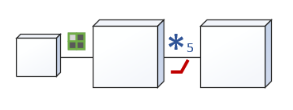
\includegraphics[scale=0.6]{image/up_conv}
          \end{center}
          \caption{Up-convolution block}
          \label{ref_sigmoid}
          \end{figure}
      \end{center}
    
    \item Up-projection: dựa trên cơ sở của up-convolution, đồng thời, up-projection cũng kế thừa ý tưởng skip connection của Resnet. Một nhánh sẽ kế thừa từ up-convolution và được gắn thêm một lớp convolution kernel size là 3$\times$3. Nhánh còn lại sẽ chỉ thực hiện convolution với kernel size 5$\times$5, trực tiếp từ kết quả của Unpooling. Với việc cộng lại kết quả từ cả 2 nhánh và thực hiện ReLU, ta có kết quả sau cùng của một uprojection block. Hình bên dưới mô tả khá rõ về cấu trúc của 1 uprojection block.
    
     \begin{center}
         \begin{figure}[H]
         \begin{center}
           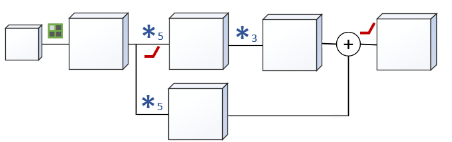
\includegraphics[scale=0.7]{image/up_projection}
          \end{center}
          \caption{Up-projection block}
          \label{ref_sigmoid}
          \end{figure}
      \end{center}
 \end{itemize}

\subsection{Dự đoán độ sâu dựa vào mẫu độ sâu thưa và một ảnh đơn với deep regression network}
Như những gì đã trình bày ở trên, nhận thấy việc chỉ dựa vào thông tin màu sắc như giá trị R, G, B để đưa ra dự đoán về độ sâu thì tính chính xác và độ tin cậy của phương pháp trên vẫn xa so với thực tế mặc dù rất nhiều nỗ lực nghiên cứu trong một thập kỉ qua dành cho phương pháp dự đoán độ sâu từ một ảnh đơn bao gồm cả những tiến bộ gần đây của kĩ thuật học sâu, cho nên ngoài việc sử dụng ảnh RGB, Ma et al.\cite{Ma2017SparseToDense} đã xem xét sử dụng thêm ảnh độ sâu thưa, đây là một bức ảnh độ sâu nhưng chỉ có một ít điểm ảnh có giá trị, còn những điểm ảnh còn lại giá trị của nó chỉ là 0. Tuy chỉ có một vài điểm có giá trị nhưng những thông tin bổ sung này đóng vai trò cực kì quan trọng giúp cho mạng CNN cải thiện đáng kể kết quả dự đoán của mình.
\subsubsection{Kiến trúc CNN của mạng deep regression network}
Kiến trúc mạng CNN của Ma et al.\cite{Ma2017SparseToDense} giống như mạng FCRN của Laina et al.\cite{laina2016deeper}, nhưng khác với FCRN thì deep regression network (DRN) của Ma còn dùng thêm ảnh độ sâu thưa, nên đầu vào của DRN là một ảnh RGB-D có channel là 4 tương ứng với 4 giá trị R, G, B và D là thông tin độ sâu tại điểm ảnh đó. Chi tiết kiến trúc được thể hiện ở hình bên dưới.
\begin{center}
         \begin{figure}[H]
         \begin{center}
           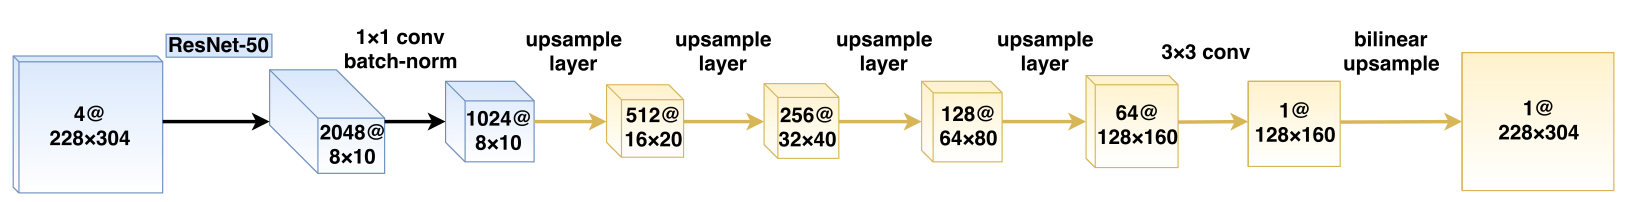
\includegraphics[scale=0.28]{image/Manet}
          \end{center}
          \caption{Kiến trúc CNN cho tập dữ liệu NYUv2 dựa trên Laina\cite{laina2016deeper}. Các khối chính là feature maps với chiều được biểu diễn bằng $\#channel@height\times width$. Các khối màu xanh là các lớp encoding bao gồm ResNet\cite{KHe2015} và 1$\times$1 convolution. Các lớp màu vàng gồm 4 lớp upsampling, một lớp 3$\times$3 convolution và một phép bilinear upsample để nâng độ phân giải về ban đầu}
          \label{ref_sigmoid}
          \end{figure}
 \end{center}

\subsubsection{Depth sampling}
Ở đây nhóm sẽ nói về chiến lược lấy mẫu để sinh ra ảnh độ sâu thưa từ ảnh độ sâu thực tế mà ta có (ground truth).\\

Trong suốt quá trình huấn luyện, ảnh độ sâu thưa $D$ sẽ được lấy mẫu ngẫu nhiên từ ảnh độ sâu thực tế $D^{*}$. Cụ thể, với mỗi một số mẫu độ sâu $m$ (cố định trong suốt quá trình huấn luyện), chúng ta tính xác suất Bernoulli $p = \frac{m}{n}$, mà $n$ là tổng số điểm ảnh hợp lệ của $D^{*}$. Điểm ảnh hợp lệ ở đây là những điểm ảnh có giá trị độ sâu không vượt quá một giá trị cho trước (giá trị này được thiết lấp cố định lúc huấn luyện). Tiếp theo, với mỗi điểm ảnh $\left (i, j \right)$,
\begin{center}
$\textit{D}\left ( i,j \right ) = \begin{cases}
 & D^{*}\left (i,j \right ),\hspace{.5cm} \text{với xác suất }  p\\ 
 & 0, \hspace{1.7cm} \text{trường hợp khác} 
\end{cases}$

\end{center}

Với chiến lược lấy mẫu này thì số lượng điểm ảnh có giá trị độ sâu khác 0 sẽ biến đổi đối với mỗi mẫu huấn luyện (training sample) xung quanh giá trị trung bình $m$. Mục đích của nó còn giúp tăng lượng dữ liệu huấn luyện giống như kĩ thuật data augmentation được trình bày sau đây.

\subsubsection{Data augmentation}

Để tăng lượng dữ liệu cho tập huấn luyện thì Ma et al.\cite{Ma2017SparseToDense} đã dùng nhiều phương pháp chuyển đối dữ liệu gốc một cách ngẫu nhiên trong quá trình huấn luyện đối với mỗi mẫu (trainning sample) tham gia.\\
Các phương pháp dưới đây áp dụng cho cả ảnh màu và ảnh độ sâu
\begin{itemize}
\item Rotation: quay một góc ngẫu nhiên $r$ $\in$ [5, -5]
\item Scale:  Nâng độ phân giải lên một hệ số ngẫu nhiên $s$ $\in$ [1, 1.5]
\item Centercrop: Chúng ta sẽ tiến hành crop trung tâm từ bức ảnh để độ phân giải của mỗi input là như nhau.
\item Flips: Ở đây ta sẽ đổi chiều bức ảnh theo chiều ngang với xác suất là 0.5
\end{itemize}
Riêng đối với ảnh màu ta còn chỉnh độ sáng, tương phản bằng các hệ số $k_{i} \in $ [0.6, 1.4] và chuẩn hóa bằng cách chia tất cả giá trị R, G, B cho 255.

\subsubsection{Hàm đo độ lỗi}
Với bài toán hồi quy thì hàm đo độ lỗi (loss function) chuẩn dùng trong qúa trình tối ưu là hàm trung bình bình phương lỗi (mean squared error) giữa giá trị thực tế y và giá trị dự đoán $y^{*}$: $L_{2}\left(y^{*} - y\right)$ = $\left \|y^{*} - y \right \|^{2}$. Hàm $L_{2}$ có ý nghĩa như sau, nếu giá trị lỗi càng lớn thì các thành phần gây ra lỗi sẽ bị phạt thật nặng để giảm lỗi. Nhưng với bài toán này Ma et al.\cite{Ma2017SparseToDense} đã cho thấy kết quả từ việc sử dụng $L_{2}$ không được tốt.\\
Một lựa chọn phổ biến khác là hàm lỗi berHu được Laina et al.\cite{laina2016deeper} sử dung:
\begin{center}
$\textit{B}\left ( e \right ) = \begin{cases}
 & \left | e \right |,\hspace{.8cm} \text{nếu}  \left | e \right | \leq  c\\ 
 & \frac{e^{2} + c^{2}}{2c}, \hspace{.4cm} \text{nếu} \left | e \right | >  c
\end{cases}$

\end{center}
Với $e = y_i^{*} - y_i$, và tại mỗi bước gradient descent, ta có $c = \frac{1}{5}\max_i\left(\left |y_i^{*} - y_i \right | \right)$, ta xét $i$ là toàn bộ điểm ảnh trên mỗi ảnh tại bó hiện tại (current batch). Ta có thể thấy được hàm berHu sẽ trở thành hàm trung bình trị tuyệt đối lỗi $L_1$ (mean absolute error) nếu như $ e \leq c$, và nó sẽ xấp xỉ $L_2$ khi lỗi vượt qua ngưỡng c, nhưng hàm này vẫn có đạo hàm tại c. Về mặt trực giác ta thấy khi một điểm ảnh có $e$ nhỏ thì berHu là hàm $L_1$ và thông thường đạo hàm theo $L_1$ lớn hơn $L_2$ và ngược lại khi $e$ lớn thì berHu xấp xỉ hàm $L_2$ và đạo hàm theo $L_2$ lại nhỏ hơn $L_1$, điều này giúp nó hội tụ tốt hơn. Nhưng nó cũng đòi hỏi chi phí tính toán lớn hơn để tìm ra hằng số c.\\

Trong những thí nghiệm của mình Ma at el. \cite{Ma2017SparseToDense} đã cho thấy $L_1$ đạt kết quả tốt hơn một chút so với berHu, nên nhóm đã chon $L_1$ làm lựa chọn mặc định vì sự đơn giản cũng như chi phí tính toán thấp hơn so với berHu.



\section{Ước lượng khoảng cách vật thể}

Như nhóm đã đề cập từ trước, để có thể ước lượng được khoảng cách vật thể từ một bức ảnh, thì nhiệm vụ đầu tiên, đó chính là phát hiện đó là vật thể gì, vật thể đó ở vị trí nào trong ảnh, đồng thời phải bao đóng và phân đoạn đối tượng đó. Đây là một bài toán kinh điển trong mảng thị giác máy tính và gây khó khăn cho nhiều nhà nghiên cứu. Là con người, chúng ta có thể dễ dàng nhìn, và biết được chúng ta đang nhìn gì, đồng thời có thể ước lượng được khoảng cách những vật đó cách chúng ta bao xa dựa trên kinh nghiệm. Nhưng với một cỗ máy, để thực hiện được nhiệm vụ trên đòi hỏi nhiều công nghệ, cũng như kết hợp nhiều kết quả nghiên cứu. Hiện nay, đã có nhiều mô hình cho kết quả rất tốt trong việc phát hiện, bao đóng và phân đoạn vật thể: SSD, Mask RCNN ... 

% Nói cách khác, chúng ta sẽ chỉ tập trung vào những bao đóng, phân đoạn chứa vật thể để có thể tối ưu hóa độ chính xác của việc ước lượng khoảng cách, giảm việc bị ảnh hưởng của những thông tin ko liên quan đến vật thể như môi trường...

\subsection{Phát hiện, bao đóng và phân đoạn vật thể}

Trong những mô hình thực hiện nhiệm vụ phát hiện, bao đóng và phân đoạn vật thể mà nhóm tìm hiểu, thì Mask RCNN \cite{He2017MaskR} là một trong những mô hình tốt nhất và cho kết quả rất tốt cả về phát hiện, bao đóng vật thể lẫn phân đoạn. Do vậy, nhóm quyết định sử dụng Mask RCNN  để kết hợp với ảnh độ sâu, là kết quả từ mô hình FCRN, nhằm giải quyết mục tiêu xác định khoảng cách vật thể.\\

Từ một ảnh RGB ban đầu, Mask RCNN sẽ cho ra kết quả là bao đóng, phân đoạn từng loại vật thể có trong ảnh. Nói cách khác, dựa trên kết quả của Mask RCNN, chúng ta sẽ chỉ tập trung vào những bao đóng, phân đoạn chứa vật thể nhằm giảm thiểu việc ảnh hưởng của những thông tin không cần thiết như những vật thể không liên quan, môi trường, ...

\subsection{Ước lượng khoảng cách vật thể}

% Với kết quả thu được từ 2 mô hình Mask RCNN và FCRN, chúng ta hiện đã có được bao đóng, phân đoạn của vật thể và ảnh độ sâu của ảnh RGB. 

Hiện nay, chúng ta có thể thấy được sự đa dạng của vật thể, không chỉ về mặt số lượng mà còn về hình dáng, kích thước. Do vậy, sẽ không có một khái niệm hoàn toàn chính xác của việc đo khoảng cách vật thể. Tùy mỗi trường hợp, mỗi mục tiêu để có thể đề xuất các cách đo khác nhau. Chẳng hạn, với những vật thể nhỏ như chai nước, điện thoại, thì khoảng cách sẽ thường được ước lượng bằng khoảng từ camera đến tâm của vật thể. Mặt khác, đối với vật thể có mô hình phức tạp hơn, như cái ghế, cái bàn, thì chúng ta cần những phương thức khác nhau để có thể ước lượng được khoảng cách.\\

Ngoài ra, nếu chỉ dựa vào kết quả bao đóng vật thể, thì những thông tin của môi trường còn nằm trong bao đóng vẫn sẽ ảnh hưởng không nhỏ đến kết quả của việc ước lượng khoảng cách. Do vậy, việc kết hợp với kết quả phân đoạn vật thể của Mask RCNN là cần thiết. \\

Dựa vào kết quả của FCRN, nhóm đã có ảnh độ sâu tương ứng của ảnh màu. Mỗi vị trí trên ảnh màu sẽ có một ước lượng độ sâu tương ứng được chứa trong ảnh độ sâu. Bằng việc kết hợp các kết quả bao đóng, phân đoạn vật thể và ảnh độ sâu, nhóm đề xuất những phương án để có thể ước lượng được khoảng cách của vật thể và đánh giá, so sánh kết quả của những phương án đã đề xuất. 

\begin{itemize}

% \item \textbf{Phương án 1}: Ước lượng khoảng cách bằng các điểm nằm trong bao đóng của vật thể. Ở đây, nhóm sẽ lấy kết quả ước lượng độ sâu từ ảnh độ sâu của tất cả những điểm nằm trong bao đóng vật thể. Kết quả của phương án này nhằm đánh giá sự ảnh hưởng của thông tin môi trường nằm trong bao đóng ảnh hưởng như thế nào đối việc ước lượng khoảng cách khi so sánh với các phương án khác.

\item \textbf{Phương án 1}: Ước lượng khoảng cách bằng lấy mẫu những điểm  xung quanh tâm bao đóng của vật thể, theo phân bố Gaussian. Với cảm quan của con người, chúng ta thường ước lượng khoảng cách dựa trên tâm của vật thể. Việc lấy những điểm xung quanh tâm bao đóng theo phân bố Gaussian cũng dựa trên kinh nghiệm này. Bên cạnh đó, với việc giảm số điểm chúng ta lấy để ước lượng khoảng cách, thì các giá trị gây nhiễu từ những điểm nằm trong bao đóng nhưng không thuộc vật thể sẽ được giảm.

\item \textbf{Phương án 2}: Ước lượng khoảng cách dựa trên kết quả phân đoạn của Mask RCNN. Ở đây, nhóm sẽ lấy tất cả những điểm  mà Mask RCNN cho là thuộc về vật thể để ước lượng khoảng cách. Theo hướng tiếp cận này, việc gây nhiễu của những điểm không thuộc vật thể sẽ được loại bỏ dựa vào kết quả phân đoạn.

\item \textbf{Phương án 3}: Ước lượng khoảng cách bằng cách lấy mẫu những điểm xung quanh tâm bao đóng của vật thể theo phân phối Gaussian, trong đó những điểm này phải được Mask RCNN cho là thuộc về vật thể. Phương án này dựa trên việc kết hợp kết quả phân đoạn của Mask RCNN và việc ước lượng khoảng cách dựa trên tâm vật thể.  

\end{itemize}



